\chapter{Introduction}
\label{sec:intro}

\section{Motivation}
\label{sec:motivation}
A sequenced route query is defined as finding the shortest path from a starting point towards a possible destination, passing through multiple locations, defined by their category type. There has been significant research and proposed approaches on the topic, but there is not a developed query language to answer this types of queries. The work in this thesis has been focused on researching the topic of sequenced route queries and designing a language to enable the user to express his need in the form of a user query in a flexible manner, such as applying different constraints on the route to be found.

\textbf{Example:}

Figure \ref{fig:example} presents a small example network with four different types of point sets, illustrated with different colors. The colored circles represent the PoIs and the lines between them represent the roads, on each road there is a label with its length. There is two restaurants, a movie theater, two banks and two pharmacies. The starting points \textit{sp} is represented by a rhombus.

Suppose that a user is planning a trip to town: he first wants to go to a restaurant for lunch, then he wants to stop by a bank, then he meets a friend in the movie theater and after that he plans to have a dinner at a restaurant. In this specific scenario, the user wants to express his wish for the restaurant to be the same, because he may prefer a route where the equality of the two restaurant PoIs is more important to him than the length of the route.

With existing approaches, the user can get the shortest route \cite{OSR} or all routes that satisfy the semantic similarity and length conditions equally \cite{semanticSRQ}, but that does not guarantee the equality of the two restaurant PoIs. Also finding k optimal routes answering the user's SRQ and then filtering out the routes where the two PoIs of type restaurant are equal has proven to not always generate a result, which is why in this thesis a better optimal approach is presented.

Using Figure \ref{fig:example}, we see that the user query in the example above, when answered as an OSR query, delivers the route $(r_1, b_1, mt_1, r_2)$ with length 11 (shown with red lines in the figure), where both restaurants $r_1$ and $r_2$ are different. Our approach strives to find the optimal route, where the two restaurants are equal. It will not necessarily be shortest possible sequenced route, but it will be the shortest route out of all possible routes, where the two PoIs are equal to each other. Such route in our example graph would be $(r_1, b_1, mt_1, r_1)$ with length 12 (shown with dashed lines in the figure).

Specific constrains such as the equality in this example are proposed in the thesis as operators on the query. We modified and extended existing approaches, which answer the Optimal Sequenced Route (OSR) Query such as the Progressive Neighbor Exploration (PNE) \cite{OSR} in order to transform the complex user query and retrieve a desired result.

\begin{figure}[h]
	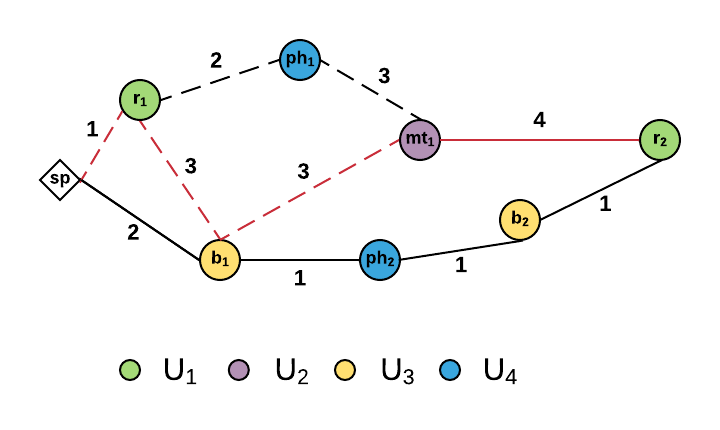
\includegraphics[scale=1]{images/Example_routes.png}
	\centering
	\caption{A network with four different types of point sets}
	\label{fig:example}
\end{figure}

\section{Problem definition}

We have a starting point and a category sequence, which constitutes the SRQ. In addition to this two query parameters, the user can define other parameters, which are applied to the route query as query operators. Such possible query operators, presented in this thesis, are the equality operator, not-equality operator, or operator and order operator. 

Then we define the \textit{Complex Route Query (CRQ)}:

\textbf{Complex route query (CRQ):} Given a starting point $sp$, a category sequence $M = (c_1, c_2, ..., c_n)$ and an operator $OPERATOR$, $Q(sp, M, OPERATOR)$ is a Complex Route (CR) Query, which searches for the optimal route $R = (r_1', r_2', ..., r_l')$, defined as a sequence of PoIs.
%Depending on which operator is applied to the query the found route $R$ follows $M$ in a way that the operator states

In Chapter \ref{sec:operators} the definitions of the separate operators are presented individually.

% e.g. performance, processing time for the trivial approach 
\section{Challenges}
When working with real-life road networks, we are usually posed with the challenge of having big datasets with many PoIs. This makes it difficult to design fast algorithms for route query problems without the need for optimizations techniques. Trivial approaches usually explore the entire dataset in order to find one optimal solution, which especially in the case of route queries can increase the time significantly. If we need to check all neighbors to one PoIs of one category and do this for all categories in order to find the shortest route from a category sequence, the time in the case of the trivial approaches increases exponentially with increase in the size of the category sequence. The \textit{Optimal Sequenced Route Query} \cite{OSR} presents the PNE approach, which solves the OSR query in metric spaces efficiently. The challenge for our task is to be able to use this designed approach to implement the proposed operators. \newline
As shown in the example in Section \ref{sec:motivation} the PNE doesn't always answer the equality operator query, therefore we modify the algorithm to serve our needs. In order to make sure that the algorithm delivers an optimal result, all routes must be checked, where two specific PoIs of one category are equal. This means that all PoIs of this category must be somehow inspected, which increases the work space significantly, which in turn spikes the processing time of the query. This poses the need for an optimization technique, such as the heuristic approach, presented in Chapter \ref{ch:EO}, to narrow the search space. \newline
The not-equality operator is an extension of the PNE algorithm, because in comparison to the equality operator, there is a greater possibility that the PNE approach finds a route with different PoIs from the same category. With a little tweak of the algorithm, it is solved by PNE without the need for an optimization technique.\newline
Furthermore, the or operator and the order operator are faced with the challenge for exponentially growing permutations, depending on the size of the query. Therefore the trivial approaches, which simply build all permutations and run PNE on them, can generate a huge work space and increase the time exponentially with the increase in the number of permutations. In our proposed approaches for these two operators we modify the PNE algorithm to be able to work on the possible permutations simultaneously, while pruning longer routes, which may be generated when the algorithm operates on the  permutations separately. In this way we shrink the search space, while also making sure, that no necessary routes are missed in the process.

% Shortly presenting the algorithms for the operators; experiment results, comparing to the baseline approach
\section{Contributions}
In this thesis, we introduce four different operators, which can be applied to a route query, and propose alternative approaches for solving them, which outperform the trivial solutions. The presented algorithms relate to the following operators: equality operator (EO), not-equality operator (NEO), or operator (OR) and order operator (ORDER). The equality operator addresses the need for flexibility, introduced in the example in Section \ref{sec:motivation}, and the not-equality solves the opposite problem, in which the user specifically wants two different PoIs of the same category type. Furthermore, the or operator represents the disjunction operator, usually present in query languages, and it gives the user the possibility to apply multiple category options to one or more route query points. Lastly, the order operator provides the user with the option to have a partially or fully not sequenced route query, where he can define zero or multiple categories to be at fixed positions in the route query sequence. \newline
The algorithms for solving the operators are largely inspired by the PNE approach, presented in the \textit{Optimal Sequenced Route Query} \cite{OSR}. For answering the equality operator query, a heuristic approach is explored, as well, for shrinking the search space and reducing the processing time. For the three of the operators (EO, OR and ORDER) baseline approaches are also introduced and compared to the proposed approaches in the experiment results. Our introduced algorithms outperform the trivial solutions in the experiments with a real dataset significantly, especially with increasing the search space with the help of different evaluation parameters, which lets us to believe that they are a meaningful way to give more flexibility to the user for different types of route queries. 

\section{Outline}
The remainder of the thesis is organized as follows: First, I review the related work that has been done on the topic of SRQ in Section 2. In Section 3 I cover the proposed operators and go into details on some of them in three separate sections for each of them: Design, Implementation and Evaluation. Finally, I conclude the thesis by summing up the progress made on the subject and discuss future work.